\documentclass[10pt,bahasa]{article}
\usepackage[a4paper]{geometry}
\geometry{verbose,tmargin=1.5cm,bmargin=1.5cm,lmargin=1.5cm,rmargin=1.5cm}
\usepackage{amsmath}
    
\setlength{\parindent}{0cm}
  
\usepackage{float}
\usepackage{graphicx}
\usepackage{enumitem}
\usepackage{hyperref}
\usepackage{url}
\usepackage{xcolor}
\usepackage{babel}

\usepackage{minted}
\newminted{scilab}{breaklines}

\definecolor{mintedbg}{rgb}{0.95,0.95,0.95}
\usepackage{mdframed}

\BeforeBeginEnvironment{minted}{\begin{mdframed}[backgroundcolor=mintedbg]}
\AfterEndEnvironment{minted}{\end{mdframed}}

\begin{document}

\title{Tugas Besar TF2202}
\date{}
\maketitle

Selesaikan soal-soal berikut ini dengan menggunakan Scilab.

Untuk setiap soal, Anda diberikan beberapa kode Scilab
sebagai contoh solusi dari soal yang diberikan.
Meskipun demikian, Anda tetap harus melengkapinya dengan beberapa
bagian penting sesuai dengan algoritma yang sudah Anda pelajari di kelas.

Kode Anda nantinya tidak harus sama persis dengan kode yang diberikan.
Anda dapat menambahkan fitur-fitur lain yang Anda anggap perlu.


%====================================
\section{Persamaan diferensial biasa}
%====================================

\subsection{Perbandingan beberapa metode numerik untuk persamaan diferensial biasa}

Carilah solusi numerik dari persamaan diferensial berikut
\begin{equation}
y''(t) + y(t) = 0
\end{equation}
dengan syarat awal
\begin{equation}
y(0) = 0, \hspace{0.5cm} y'(0) = 1
\end{equation}
pada interval $0 \leq t \leq 50$.

Bandingkan solusi yang diperoleh dengan solusi analitik:
\begin{equation}
y(t) = \sin(t)
\end{equation}

Gunakan menggunakan metode-metode berikut ini untuk mencari solusi numeriknya.
\begin{itemize}
\item Euler
\item Euler dengan prediktor-korektor (Runge-Kutta orde-2)
\item Runge-Kutta orde-4
\end{itemize}

Dari solusi numerik yang didapatkan, buatlah (1) plot antara $y$ dan $y'$
dan (2) plot antara $t$ dan $y$.

\subsection*{Kode Scilab}

Metode Euler file (file: \texttt{ode\_euler.sce})

\begin{scilabcode}
function [t,y] = ode_euler(f,tspan,y0,N)
  //
  // ODE dideskripsikan dengan handle fungsi f yang menerima masukan t dan y
  // (lihat contoh)
  //
  // tspan(1) : t awal
  // tspan(2) : t akhir
  //
  // N: jumlah selang t
  
  // diskritisasi t
  h = (tspan(2) - tspan(1))/N
  t = tspan(1) + [0:N]'*h
    
  // cek y0, transpos jika diperlukan
  if size(y0,1) ~= 1
    if size(y0,2) > 1
      y0 = y0'
    end
  end
  
  // cek dimensionalitas dari ODE
  Ndim = size(y0,2)
  y = zeros(N+1,Ndim)
    
  // set nilai awal
  y(1,:) = y0
  
  // Tuliskan metode Euler di sini (BONUS=sudah diberikan)
  for k = 1:N
    y(k+1,:) = y(k,:) + h*f( t(k), y(k,:) )
  end
  
endfunction  
\end{scilabcode}

Contoh penggunaan fungsi \verb|ode_euler|

\begin{scilabcode}
exec("ode_euler.sce",-1)

// definisi ODE
function f = dy(t,y)
  f(1) =  y(2)
  f(2) = -y(1)
  f = f'  // konvensi: ubah menjadi vektor baris
endfunction
  
tspan = [0 50]
y0 = [0 1]

// isi parameter numeriknya di sini
h = 0.05
N = (tspan(2) - tspan(1))/h

[t,y] = ode_euler( dy, tspan, y0, N )

// plot dan sebagainya
plot( t, y(:,1) )  // t vs y1
plot( t, y(:,2) )  // t vs y2
plot( y(:,1), y(:,2) ) // y1 vs y2
\end{scilabcode}


Metode Euler dengan prediktor-korektor: (file: \texttt{ode\_euler\_PC.sce})

\begin{scilabcode}
function [t,y] = ode_euler_PC(f,tspan,y0,N)
  
  // sama dengan ode_euler
  // ....

  // Ini bagian yang berbeda, lengkapi utk metode Euler PC (Runge-Kutta orde 2)
  for k = 1:N
    // lengkapi kode ini
    // ....
  end
endfunction
\end{scilabcode}

Metode Runge-Kutta orde 4 (file: \texttt{ode\_RK4.sce})

\begin{scilabcode}
function [t,y] = ode_RK4(f,tspan,y0,N)
  
  // sama dengan ode_euler
  // ...

  // Lengkapi dengan metode Runge-Kutta orde 4
  for k=1:N
    f1 = ...
    f2 = ...
    f3 = ...
    f4 = ...
    y(k+1,:) = y(k,:) + (f1 + 2*(f2+f3) + f4)/6
  end
endfunction
\end{scilabcode}


%============================
\subsection{Gerakan pendulum}
%============================

Gerak suatu pendulum dapat dinyatakan dengan persamaan diferensial:
\begin{equation}
\theta''(t) = -\frac{g}{L}\sin(\theta(t)) - k\theta'(t)
\end{equation}
dengan syarat awal
\begin{equation}
\theta(0) = \theta_0, \hspace{0.5cm} \theta'(0) = 0
\end{equation}

\begin{figure}[H]
\centering
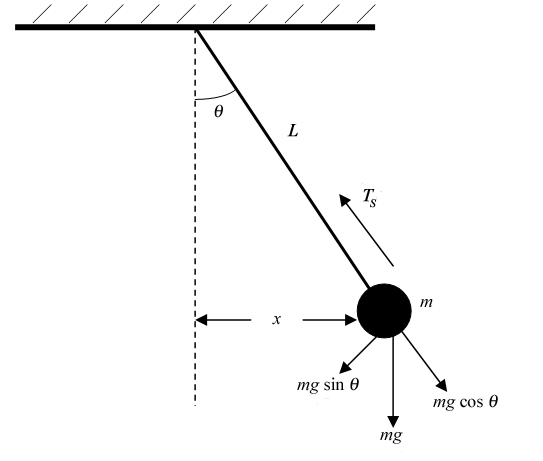
\includegraphics[scale=0.4]{images/pendulum.png}
\par
\caption{Pendulum sederhana}
\end{figure}

Dalam persamaan tersebut $\theta$ menyatakan simpangan pendulum,
$\theta_0$ menyatakan simpangan awal pendulum,
$g$ menyatakan percepatan gravitasi, $L$ menyatakan panjang benang pendulum,
dan $k\theta'$ menyatakan suku redaman (gesekan) yang berbanding lurus
dengan kecepatan $\theta'$ ($k$ adalah bilangan positif).

\begin{enumerate}[label=(\alph*)]
\item Cari solusi $\theta(t)$ untuk kasus $k=0$ untuk simpangan awal $\theta_0 = 0.1, \pi/5$
dan 3.0.
\item Carilah solusi $u(t)$ untuk kasus $k = 0.1, 0.3, 0.5$ dan 0.8 untuk
simpangan awal yang sama.
\end{enumerate}

\subsection*{Kode Scilab}

Dengan menggunakan metode Runge-Kutta orde 4 yang telah dibuat
pada bagian sebelumnya.

\begin{scilabcode}
exec("ode_RK4.sce",-1)

// parameter dan konstanta
global g
global L
global k

g = ... // percepatan gravitasi
L = ... // panjang tali
k = ... // suku redaman

// Syarat awal untuk kecepatan
du0 = 0.0

t0 = 0.0
tmax = 20.0
// masukkan parameter numerik yang Anda pikir cukup baik
delta_t = 0.01
N = (tmax - t0)/delta_t

// Deskripsi ODE dalam function
function f = soal_02(t,u)
  global g
  global L
  global k
  //  
  f(1) =  ... // lengkapi
  // k*u(2) adalah suku redaman
  f(2) = ... // lengkapi
  f = f'  // konvensi, ubah menjadi vektor baris
endfunction

[t,u1] = ode_RK4( soal_02, [t0 tmax], [0.1 du0], N)
// ... teruskan untuk syarat awal yang lain
// ... plot solusi
\end{scilabcode}



\section{Persamaan transfer kalor}

Hitung solusi numerik dari
\begin{equation}
\frac{\partial^2 u(x,t)}{\partial x^2} = \frac{\partial u(x,t)}{\partial t}
\end{equation}
untuk $0 \leq x \leq 1$ dan $0 \leq t \leq 0.1$ dengan syarat awal
\begin{equation}
u(x,0) = \sin(\pi x)
\end{equation}
dan syarat batas
\begin{equation}
u(0,t) = 0,\hspace{0.5cm} u(1,t) = 0
\end{equation}
Gunakan metode Euler eksplisit, Euler implisit dan Crank-Nicolson serta
bandingkan hasilnya.
Buat juga animasi (dalam format GIF) yang menggambarkan perubatan profil
suhu terhadap waktu.

\subsection*{Solusi}

Metode Euler eksplisit file: \verb|heat_1d_euler_exp.sce|

\begin{scilabcode}
function [u,x,t] = heat_1d_euler_exp(a,xf,T,initialTemp,bx0,bxf,Nx,Nt)
  // bangun grid x dan t
  dx = xf/Nx
  x  = [0:Nx]'*dx
  //
  dt = T/Nt
  t  = [0:Nt]*dt
  // Syarat awal
  for i = 1:Nx+1
    u(i,1) = initialTemp(x(i))
  end
  // Syarat batas
  for it = 1:Nt+1
    u([1 Nx+1],it) = [bx0(t(it)); bxf(t(it))]
  end
  //
  // persamaan yang ada di slide mungkin menggunakan notasi yang berbeda
  // silakan ganti jika Anda mau
  //
  r  = a*dt/dx/dx
  r1 = 1 - 2*r
  
  // Tampilkan pesan jika solusi numerik tidak stabil
  if r > 0.5
    printf("\nheat_1d_euler_exp:\n")
    printf("WARNING: r is larger than 0.5: %f\n", r)
    printf("WARNING: solution is not stable\n\n")
  else
    printf("\nheat_1d_euler:\n")
    printf("r = %f >= 0.5\n", r)
    printf("The solution should be stable\n\n")
  end
  
  for it = 1:Nt
    for i = 2:Nx
      u(i,it+1) = ... // lengkapi
    end
  end
endfunction  
\end{scilabcode}

Contoh pemanggilan dengan metode eksplisit

\begin{scilabcode}
exec("heat_1d_euler_exp.sce",-1)

// initial condition (function of x)
function T = it0(x)
  T = ... // lengkapi
endfunction

// boundary condition (function of t)
function T = bx0(t)
  T = 0.0
endfunction

function T = bxf(t)
  T = 0.0
endfunction

function T = analytic_solution(x,t)
  T = sin(%pi*x)*exp(-%pi*%pi*t)
endfunction

// fungsi pembantu, mengubah integer menjadi string
// dengan 'padded'-zeros
function str = to_string(i)
  if i < 10
    str = "000" + string(i)
  elseif i < 100
    str = "00" + string(i)
  elseif i < 1000
    str = "0" + string(i)
  else
    str = string(i)
  end
endfunction

// fungsi
function plot_to_png(u,x,t,prefix)
  Nt = length(t)-1
  for it = 1:Nt+1
    clf()
    plot(x,u(:,it))
    set(gca(), "data_bounds", [0,1,0,1]) // set batas
    strt = "t = " + string(t(it))
    xstring(0.8,0.9,strt) // menampilkan waktu
    xs2png(gcf(), prefix + to_string(it) + ".png") // ubah ke png
    printf("Done output solution for t = %f\n", t(it))
  end
endfunction

// parameter (diberikan di soal)
a  = 1
xf = 1
T  = 0.1

// coba bereksperimen dengan mengubah nilai-nilai berikut
Nx = 25
Nt = 100

// Explicit Euler
[u1,x,t] = heat_1d_euler_exp( a, xf, T, it0, bx0, bxf, Nx, Nt )
plot_to_png(u1,x,t,"TEMP_exp_")

u_analytic = analytic_solution(x,t)

// Error dibandingkan dengan solusi analitik
NxNt = Nx*Nt
err1 = norm( (u1 - u_analytic) )/NxNt

printf("Error dengan metode eksplisit = %f\n", err1)
\end{scilabcode}

Metode Euler implisit

\begin{scilabcode}
function [u,x,t] = heat_1d_euler_imp(a,xf,T,initialTemp,bx0,bxf,Nx,Nt)

  // mirip dengan heat_1d_euler_exp
  
  r  = a*dt/dx/dx
  r2 = 1 + 2*r
  
  // Build matrix A
  for i = 1:Nx-1
    A(i,i) = ... // lengkapi
    if i > 1
      A(i-1,i) = ... // lengkapi
      A(i,i-1) = ... // lengkapi
    end
  end
  
  // Time-stepping, menyelesaikan persamaan linear
  for k=2:Nt+1
    b = [r*u(1,k); zeros(Nx-3,1); r*u(Nx+1,k)] + u(2:Nx,k-1);
    u(2:Nx,k) = ... // lengkapi
  end
  
endfunction  
\end{scilabcode}

Metode Crank-Nicolson

\begin{scilabcode}
function [u,x,t] = heat_1d_CN(a,xf,T,initialTemp,bx0,bxf,Nx,Nt)
  
  // mirip dengan heat_1d_euler_exp
  
  r  = a*dt/dx/dx
  r1 = 2*(1-r)
  r2 = 2*(1+r)
  
  // Matriks A
  A = zeros(Nx-1,Nx-1)
  for i = 1:Nx-1
    A(i,i) = ... // lengkapi
    if i > 1
      A(i-1,i) = ... // lengkapi
      A(i,i-1) = ... // lengkapi
    end
  end
  
  // Matriks B
  B = zeros(Nx-1,Nx-1)
  for i = 1:Nx-1
    B(i,i) = ... // lengkapi
    if i > 1
      B(i-1,i) = ... // lengkapi
      B(i,i-1) = ... // lengkapi
    end
  end

  // Time-steping, solve linear equation
  for it = 2:Nt+1
    b = B*u(2:Nx,it-1)
    u(2:Nx,it) = ... // lengkapi
  end
  
endfunction  
\end{scilabcode}

Uji juga dengan menggunakan metode implisit dan Crank-Nicolson.



\end{document}
